\documentclass[11pt,a4paper]{article}
\usepackage[utf8]{inputenc}
\usepackage[T1]{fontenc}
\usepackage{amsmath}
\usepackage{amsfonts}
\usepackage{amssymb}
\usepackage[left=3.0cm, right=3.0cm, top=3.0cm, bottom=3.0cm]{geometry}
\usepackage{xcolor}
\usepackage{graphicx}
\usepackage{caption}
\usepackage{subcaption}

% include code listings
\usepackage{listings}

% Defining colors for syntax highlighting
\definecolor{codegreen}{rgb}{0,0.6,0}
\definecolor{codegray}{rgb}{0.5,0.5,0.5}
\definecolor{codepurple}{rgb}{0.58,0,0.82}
\definecolor{backcolour}{rgb}{0.95,0.95,0.92}

\lstdefinestyle{mystyle}{
	backgroundcolor=\color{backcolour},   
	commentstyle=\color{codegreen},
	keywordstyle=\color{magenta},
	numberstyle=\tiny\color{codegray},
	stringstyle=\color{codepurple},
	basicstyle=\ttfamily\footnotesize,
	breakatwhitespace=false,         
	breaklines=true,                 
	captionpos=b,                    
	keepspaces=true,                 
	numbers=left,                    
	numbersep=5pt,                  
	showspaces=false,                
	showstringspaces=false,
	showtabs=false,                  
	tabsize=2
}

\lstset{style=mystyle}
\captionsetup[lstlisting]{font={scriptsize}}

% header and footer
\usepackage{fancyhdr}
\pagestyle{fancy}
\fancyhf{}
\lhead{Michele Guadagnini}
\rhead{\today}
\lfoot{Ex 5 - Quantum Information and Computing 2020/2021}
\rfoot{Page \thepage}

\author{Michele Guadagnini - ID 1230663}
\title{\textbf{Exercise 5 \\ Eigenproblem \& Random Matrix Theory}}
\date{\today}

%File names must include your name, exercise number and codewords REPORT, and CODE.
%Example: Ex2-Rossi-REPORT.pdf
%The maximum length of the report is five pages
\begin{document}
\maketitle

\vspace{20pt}
\begin{abstract}
	The aim of this exercise is to study the distribution of normalized spacings of eigenvalues for different types of random matrices. 
	The two types considered in this work are: \textit{Hermitian} matrix and \textit{Diagonal} matrix.
\end{abstract}

\section{Theory} %Explain briefly the theory you have based your solution on.
A complex square matrix is \textit{Hermitian} if it is equal to its own conjugate-transpose matrix. 
It means that the element $a_{i,j}$ is the complex conjugate of $a_{j,i}$, so the main diagonal contains only real values, and it has real eigenvalues.
The normalized spacings $s_i$ between eigenvalues sorted in increasing order are defined as:
\begin{equation}
	s_i = \frac{\Delta\lambda_{i}}{\overline{\Delta\lambda}} \quad with \quad \Delta\lambda_{i} = \lambda_{i+1} - \lambda_i
\end{equation}
where $\overline{\Delta\lambda}$ represents the average of $\Delta\lambda_{i}$.

The normalized spacings of an random Hermitian matrix are expected to have a distribution that can be modeled with four parameters as:
\begin{equation}
	P(s) = as^\alpha \exp(-bs^\beta)
	\label{eq:fitmodel}
\end{equation}

\section{Code Development} %Introduce strategies, tests, and report debugging problems, compilations options

\subsection{Design and Implementation}

The code implementation started from building up the module \textit{NormalizedSpacings} that contains all the subroutines needed for the calculation of eigenvalues and spacings. It is implemented in the file \textit{Ex5-Guadagnini-NormSpacings-CODE.f90}.
In particular the computations has been divided in the following sub-tasks:
\begin{itemize}
	\item \textit{RandInitHermitianMat}: it initializes the hermitian matrix as a double complex upper triangular matrix with real diagonal, since lower triangular elements can be calculated from the upper ones. Real and Imaginary part are set to be in $[10 , -10]$ range.
	\item \textit{HermEigenvalues}: it computes the eigenvalues of the hermitian matrix by using the \textit{ZHEEV} subroutine from \textit{LAPACK} library.
	\item \textit{NormSpacings}: it computes the spacings from an array of eigenvalues, that must be previously ordered.
	\item \textit{ComputePDF}: it computes the probability distribution from an array of double precision numbers. It receives as input also the number of bins, the extremes of the histogram and two arrays where to save the results, one for the middle values of the bins and one for the computed probabilities. 
	\item \textit{PrintColumnsOnFile}: it prints in two columns the results, in the first the bin centers, in the second the corresponding probabilities.
\end{itemize}

All these subroutines are then used in the main program in the file \textit{Ex5-Guadagnini-CODE.f90}.

The first part of the program reads the size of the matrices and the number of bins from the command line arguments. It also reads the debug flag if present.

Once set the matrix size and the number of bins the program continues with the initialization of the diagonal matrix. 
The diagonal elements are sampled with uniform distribution between $10$ and $-10$ and sorted in increasing order by using the subroutine \textit{DLASRT} from \textit{LAPACK}. 
Then, the array of eigenvalues is passed to \textit{NormSpacings} subroutine and finally the subroutine \textit{ComputePDF} is called with the computed spacings, the number of bins, the appropriate extremes for the histogram and the arrays to store the results.

The last part of the program is about the hermitian matrix spacings. 
The structure of this part is very similar to the previous one, except for the matrix initialization and diagonalization. 
These tasks are done by the dedicated subroutines \textit{RandInitHermitianMat} and \textit{HermEigenvalues}. 

It is useful to mention also that the debugger module has been included and used in this program as in the previous exercises. 

Once produced the data the implementation proceeded by writing down the \textit{gnuplot} script to do plots and fits. 
The script is structured to receive as input the name of the file containing the data and the maximum x and y values to set the proper range of the plot. 
The main steps of the script are the definition of the fit model according to Eq. \ref{eq:fitmodel}, the plot of distribution and fitted model and the residuals plot. They are reported in the following listing:
\lstinputlisting[language=BASH, linerange={9-11}, firstnumber={9}]{Ex5-Guadagnini-SpacingsFit.gnu}
\lstinputlisting[language=BASH, linerange={31-41}, firstnumber={31}, caption=More relevant parts of the \textit{gnuplot} script.]{Ex5-Guadagnini-SpacingsFit.gnu}

\subsection{Debug and Test}

The program has been firstly tested with the default matrix size that is set to be $200$. With this size, and also greater ones, the program worked fine (the greatest size that has been tested to work is $5000$), even with all the optimization flags up to \textit{-O3}. 
With a larger matrix ($10000$) the program returned only some non-zero values for the probabilities of the spacings distribution. 
It happened with all the optimization flags but only for the diagonal matrix spacings when it was computed after the hermitian matrix spacings. 
The solution was to reverse the order of computation, calculating firstly the diagonal matrix spacings and then the hermitian ones, suggesting the problem to be related to memory allocation or management.
This way the program works fine also for very large matrices with up to \textit{-O3} flag, while with \textit{-Ofast} option the program returns bad results (some $NaN$ values).

In the end the program has been compiled and executed for a matrix of size $10000$ and a number of bins of $150$:
\begin{lstlisting}[language=BASH,numbers=left]
gfortran *CODE.f90 -o RandMatTheory.x -lblas -llapack -O3
./RandMatTheory.x 10000 150
\end{lstlisting}

\section{Results} %Present data and explain your results.

The obtained distributions has been fitted according to the model in Eq. \ref{eq:fitmodel}. The resulting parameters for both diagonal and hermitian matrices are reported in Table \ref{tab:fitpars}.
\begin{table}[h]
	\begin{center}
		\begin{tabular}{ccc}
			\hline
			         & \textbf{Diagonal spacings} & \textbf{Hermitian spacings} \\ 
			\hline
			   \textbf{$a$}   &   1.7 $\pm$ 0.1   &     17 $\pm$ 7     \\
			\textbf{$\alpha$} & 0.027 $\pm$ 0.033 &   2.6 $\pm$ 0.2    \\
			   \textbf{$b$}   &   1.0 $\pm$ 0.1   &   3.0 $\pm$ 0.4    \\
			\textbf{$\beta$}  &  1.03 $\pm$ 0.07  &   1.3 $\pm$ 0.1    \\ 
			\hline
		\end{tabular}
	\end{center}
	\caption{Results of the spacings distributions fits.}
	\label{tab:fitpars}
\end{table} 
It can be easily noticed that the obtained parameters are very different for the two fits. 
In particular the parameter $a$ is much bigger for the hermitian spacings fit, though it has a very large error ($42\%$), and the parameter $\alpha$ is $2.6$ in the hermitian spacings fit, while it is very close to $0$ for the diagonal fit (actually, considering the error, its value is surely compatible with zero).
This suggests that the diagonal spacings distribution has a shape much more similar to a simpler exponential decay, as can be seen in Figure \ref{fig:diag}.
The residuals plots in Figure \ref{fig:diag} and \ref{fig:herm} together with the \textit{fit.log} file content confirms the goodness of the fits.

% figure and subfigures
\begin{figure}
	\centering
	\begin{subfigure}{0.9\textwidth}
		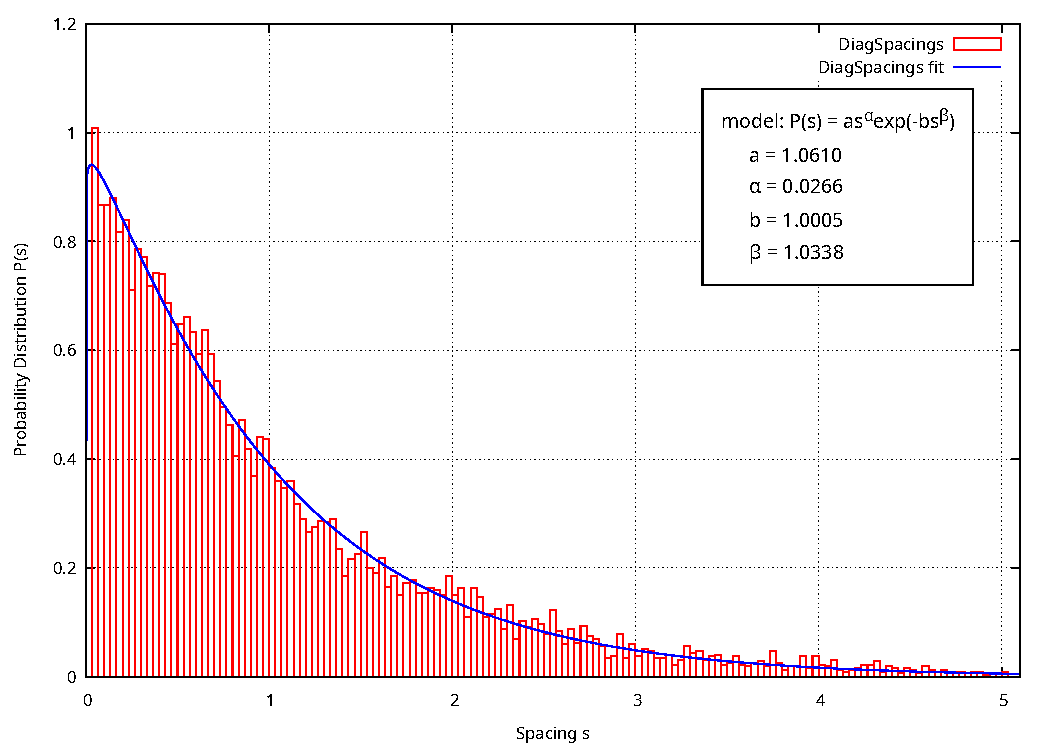
\includegraphics[width=1\linewidth]{Fit_DiagSpacings.pdf}
	\end{subfigure}
	\begin{subfigure}{0.9\textwidth}
		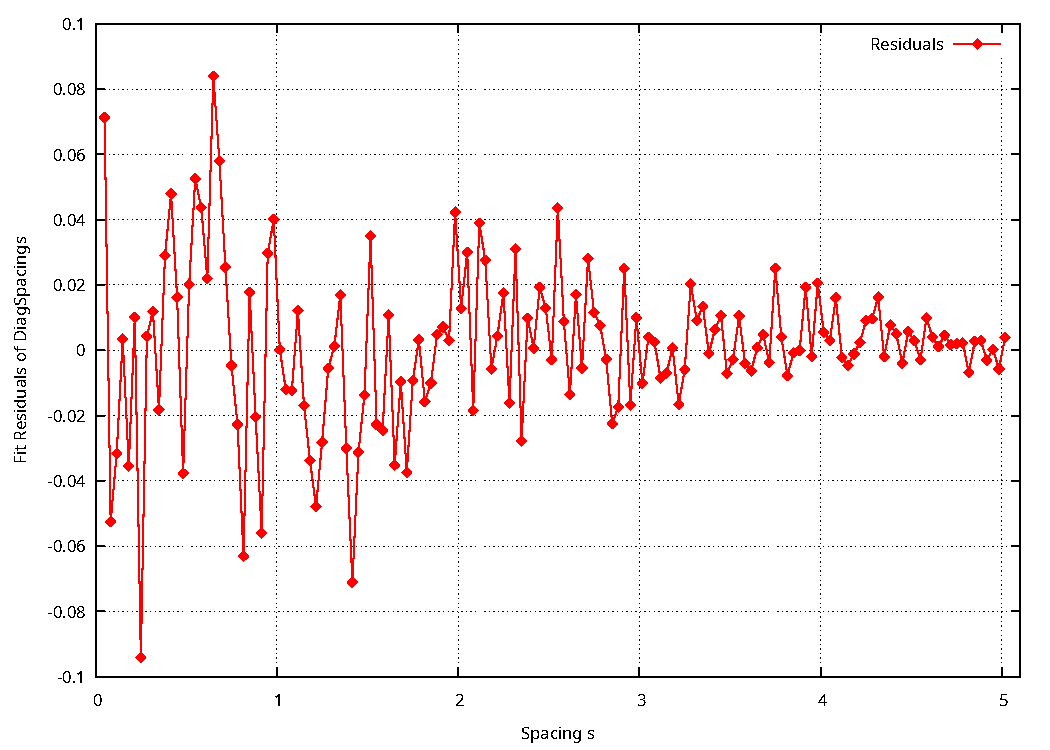
\includegraphics[width=1\linewidth]{Res_DiagSpacings.pdf}
	\end{subfigure}
	\caption{Fit of the distribution of diagonal matrix spacings and related residuals plot.}
	\label{fig:diag}
\end{figure}

\begin{figure}
	\centering
	\begin{subfigure}{0.9\textwidth}
		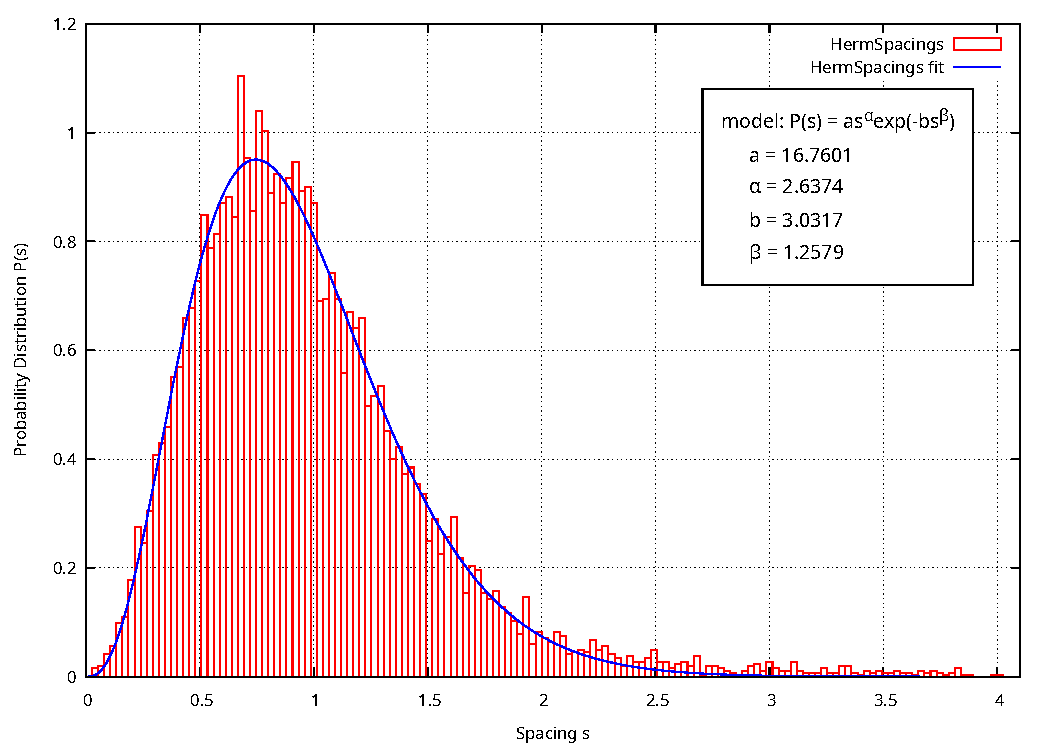
\includegraphics[width=1\linewidth]{Fit_HermSpacings.pdf}
	\end{subfigure}
	\begin{subfigure}{0.9\textwidth}
		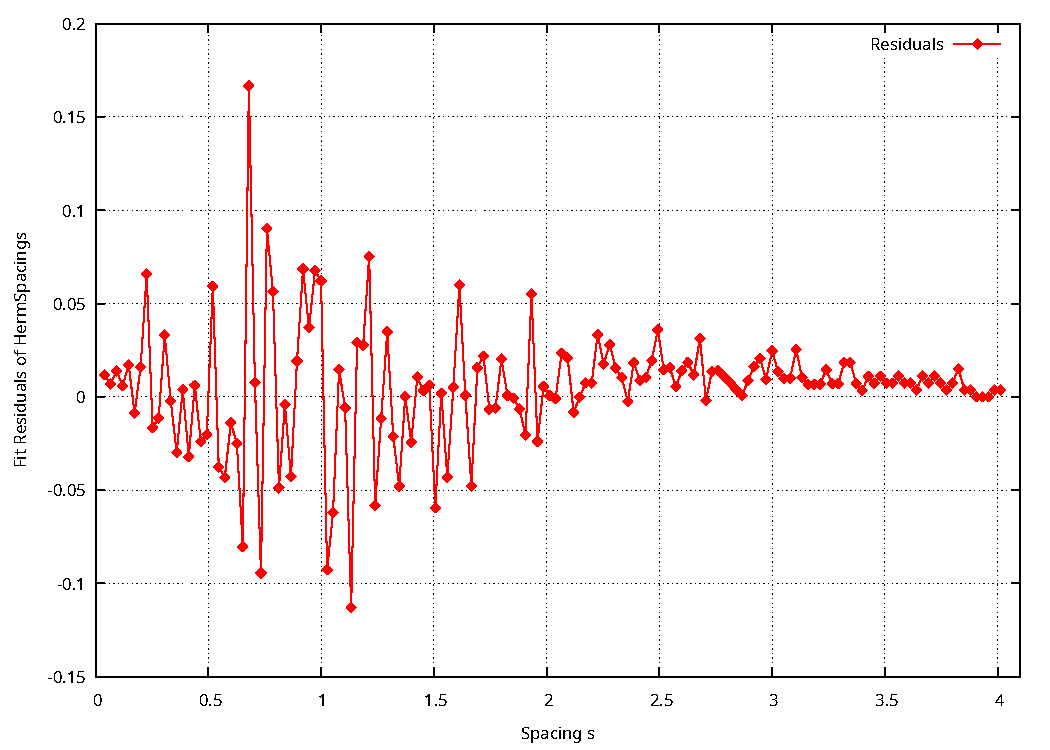
\includegraphics[width=1\linewidth]{Res_HermSpacings.pdf}
	\end{subfigure}
	\caption{Fit of the distribution of hermitian matrix spacings and related residuals plot.}
	\label{fig:herm}
\end{figure}

\section{Self-evaluation} %What have you learned? What can be done next? What went wrong and why?

Things learned while completing this assignment are to use \textit{LAPACK} library in a program and in particula the subroutine \textit{ZHEEV} to diagonalize a hermitian matrix.

The first thing to be done next is to complete the optional assignments (local average spacings and the average <r> computation).
It would have been useful to separate spacings computation and histogram building in different programs. This would provide more flexibility.
It would have been better also to do the computation multiple times with smaller matrices in order to increase available data while keeping the same computation time and also to be able to estimate a statistical error over distribution points.
	
\end{document}
